\documentclass[11pt]{article}

\usepackage[margin=1in]{geometry}
\usepackage{amsmath,amssymb,amsthm,mathtools}
\usepackage{booktabs,array,tabularx}
\usepackage{enumitem}
\usepackage{tikz}
\usetikzlibrary{arrows.meta,positioning,calc}
\usepackage{microtype}
\usepackage{natbib}
\usepackage{xcolor}
\usepackage[colorlinks=true,allcolors=blue!45!black]{hyperref}

\newtheorem{theorem}{Theorem}
\newtheorem{proposition}{Proposition}
\newtheorem{lemma}{Lemma}
\newtheorem{corollary}{Corollary}
\theoremstyle{definition}
\newtheorem{definition}{Definition}
\theoremstyle{remark}
\newtheorem{remark}{Remark}

\newcommand{\E}{\mathbb E}
\newcommand{\calE}{\mathcal E}
\newcommand{\R}{\mathbb R}
\newcommand{\ind}{\mathbf 1}
\newcommand{\ph}{\phi}
\DeclareMathOperator*{\argmax}{arg\,max}

\title{\bfseries Announced Rescue Payments with Strategic Drivers\\
\large Commitment, Universal Rejection, and Latent Local Supply}
\author{}
\date{}

\begin{document}
\maketitle

\begin{abstract}
We study a platform that commits ex ante to a payment for a request and a
higher payment that becomes available only after universal rejection.  The
realized local driver pool is Poisson and unobserved; private-cost incumbents
simultaneously choose whether to accept now or preserve a discounted option
to wait.
The rider privately decides whether to post and, after failure, whether to
abandon, repeat, or activate rescue.  We first characterize every anonymous
symmetric pure-cutoff weak perfect Bayesian equilibrium under an arbitrary
menu, including beliefs and boundary actions.  Whenever a positive rider mass
uses marginal rescue, a small announced increase strictly raises completion
for every fresh-entry rate.  In the no-entry baseline, we prove the stronger
result that every menu has a unique cutoff.  This yields an
exact solution of the platform's full policy problem: conditional on the
first payment, the optimal rescue payment is either a reject-all boundary, a
unique tangent rescue, or an irrelevant repeat-only payment.  A Lambert-$W$
envelope reduces the global two-price problem to a continuous scalar maximum,
so an optimal menu exists.  The dynamic policy strictly dominates the
optimized flat payment whenever rider patience exceeds an endogenous
threshold; in particular, it does so for every finite market thickness when
$\beta\ge1/2$.  The gain is continuous in thickness and has an attained
interior maximum.  Driver impatience changes the thin-market order: for
$\beta>1/2$ the gain is first order in $m$ when drivers strictly discount,
but only second order at the no-discount boundary.  The thick-market rate
remains $(\log m)/m$.  We do not prove strict single-peakedness; when
$\beta<1/2$, an initial zero plateau rules it out.  A public-$N$ benchmark
separates two local mechanisms: intertemporal compensation already operates
with one incumbent, while assignment competition amplifies it with several.
\end{abstract}

\section{Introduction}
\label{sec:introduction}

Platforms often increase the payment attached to a request that remains
unfilled.  If the increase is announced in advance, it creates a commitment
problem.  A higher rescue payment makes a failed request easier to fill, but
it also makes rejection today more attractive.  Completion design must
therefore account for the strategic delay induced by the rescue policy itself.

We study a single request and two periods.  Before any private action, the
platform announces a menu $(p_1,p_2)$ with $p_2\ge p_1$.  A rider with private
value decides whether to post.  Private-cost incumbent drivers then
simultaneously accept or wait.  Waiting discounts an incumbent's terminal
net payoff by $\delta\in(0,1]$.  If at least one accepts, one is selected
uniformly.  If all reject, the rider observes only this public failure and may
abandon, repeat $p_1$, or activate $p_2$.  Incumbents can survive and fresh
drivers can enter before the terminal acceptance decision.

The information structure is central.  Market thickness $m$ is public, but
the realized incumbent count is not observed by the platform, rider, or any
individual driver.  Conditional on a focal driver being present, her rival
count remains Poisson by Palm conditioning.  Universal rejection consequently
does two jobs: it activates rescue and reveals that no incumbent below the
equilibrium cutoff accepted.  A driver's assignment probability after
accepting now is
\[
 \ph(ma)=\frac{1-e^{-ma}}{ma},
\]
whereas reaching the continuation game after waiting requires every rival to
reject, an event with probability $e^{-ma}$.  Assignment competition is one
operational wedge behind the local effect.  A second wedge is temporal:
announced escalation can compensate a waiting incumbent for discounting.
Neither wedge by itself is our mathematical contribution.

Our analysis follows the policy--response--optimization order used by
\citet{AvivPazgal2008}: fix an announced policy, solve the strategic threshold
response, and only then optimize.  The economic direction is reversed.
Forward-looking consumers in announced-markdown models wait for a lower price
and risk stockout; our suppliers wait for a higher payment and risk losing the
request to a rival.

The paper makes four contributions.  First, it gives a complete cutoff-WPBE
characterization under arbitrary survival and entry, with the Palm posterior,
failure posterior, rider continuation choices, boundary cutoffs, and
tie-breaking stated explicitly.  The assessment is conservative only within
the anonymous symmetric pure-cutoff class; it is not a worst case over every
mixed or asymmetric PBE.  We then prove a uniform local result across fresh
entry rates: if marginal rescue is active for positive rider mass, the unique
nearby cutoff moves according to an explicit coefficient and completion rises
strictly.

Second, for the uniform no-entry baseline we solve the global menu problem.
Every strict active menu has one cutoff, not merely a locally selected branch.
For a fixed $p_1$, rescue-price design becomes a strictly concave envelope.
We identify the exact reject-all, tangent-rescue, and repeat-only regimes and
then invert the fixed-price solution with the feasible root of one quadratic.
The outer problem is a continuous one-dimensional maximum, which proves
policy attainment and gives an exact optimizer correspondence.

Third, we characterize rider patience and market thickness.  Strict dynamic
gain occurs exactly for $\beta>\beta_c(m,\alpha,\delta)$, where the threshold has an
independently checkable scalar test and explicit bounds.  Since the unique
flat optimizer is below $1/2$, the sufficient condition extends to
$\beta=1/2$.  In thickness, the optimized gain is continuous, vanishes at
both endpoints, and attains a positive interior maximum.  We prove optimized
endpoint rates rather than transferring a local derivative through an
optimization.  We deliberately do not call this single-peaked: the required
global derivative theorem is unavailable, and for $\beta<1/2$ strict
single-peakedness is false because the value is initially zero.

Fourth, a public deterministic-supply benchmark separates latent information,
driver impatience, and assignment competition.  With $\delta<1$, a marginal
rescue strictly raises completion even for one known incumbent.  At
$\delta=1$, that temporal term disappears: the one-incumbent derivative is
zero and the derivative is positive exactly when $n\ge2$.  Latent Poisson
supply shapes inference and global design, but is not required for either
local mechanism.

\section{Related literature and contribution boundary}
\label{sec:literature}

We do not claim to introduce multistage bonuses or failure-contingent payment
increases.  The closest operational work is \citet{WuEtAl2022}, who optimize
multistage order-specific bonuses in meal delivery and document substantial
reductions in cancellation.  Their stage acceptance model depends on the
current bonus; it does not model a driver who strategically responds to an ex
ante announced future bonus.  Two-round broadcast and notification mechanisms
also study a second attempt after no response, but vary reach or assignment
rather than solve an announced same-request wage game
\citep{SunEtAl2020,QinEtAl2025}.

The closest behavioral work studies strategic supplier rejection.
\citet{SiggEtAl2025} model workers who reject a delivery request so that it is
reoffered at a higher payment, emphasizing labor oversupply and collective
action.  \citet{Chen2012} derives private-cost sellers' willingness to wait
for higher buyer offers when the seller count is fixed and known and the buyer
does not precommit.  Related work examines failure-contingent rewards,
rejection in anticipation of future surge, and strategic withholding of
available supply \citep{AcemogluEtAl2014,GargNazerzadeh2022,BaiEtAl2023}.
Our narrower object is the intersection of ex ante commitment, simultaneous
same-request competition, an unobserved realized rival pool, and universal
rejection as an endogenous public signal.

Finally, two-sided dynamic pricing already incorporates forward-looking
buyers and sellers.  \citet{ChenHu2020} study Poisson arrivals and strategic
waiting in a dynamic matching market.  \citet{HuHuZhu2022} obtain both
high--low and low--high two-period surge paths under rider and driver temporal
responses.  Announced and contingent pricing with strategic consumers
provides the methodological mirror \citep{AvivPazgal2008,CorreaEtAl2016}.
Relative to these papers, our policy is attached to one request, available
only after universal rejection, and optimized over the equilibrium delay it
induces among the same incumbents.

\section{Model}
\label{sec:model}

\subsection{Primitives and policy}

There is one potential request and two periods.  Market thickness $m>0$ is
public.  Before rider or driver private information is used, the platform
commits to
\[
 \mathcal P^D=\{(p_1,p_2):0\le p_1\le p_2\le1\}.
\]
The second payment is available only following first-period failure and
cannot be revised ex post.  A flat policy is $(p,p)$.  Payment is a transfer
from the rider to the selected driver.  The platform maximizes the
unconditional probability that the potential request is completed; it does
not maximize profit or welfare.

The rider has $v\sim U[0,1]$.  A period-1 completion yields $v-p_1$ and a
period-2 completion at payment $p_j$ yields $\beta v-p_j$, where
$\beta\in(0,1)$.  Incumbents have a separate discount factor
$\delta\in(0,1]$: if an incumbent waits and is selected in period 2, her
period-1-equivalent net payoff is $\delta(p_j-c)$.  A fresh entrant arrives
only in period 2 and evaluates the contemporaneous payoff $p_j-c$.  Thus
$\beta$ measures rider patience and $\delta$ measures incumbent-driver
patience; the common-discount specification is the restriction
$\delta=\beta$.  From the request perspective the incumbent count is
\[
 N^I\sim\operatorname{Pois}(m).
\]
The realization is latent to every player.  Incumbent costs are i.i.d.
$U[0,1]$ and remain fixed across periods.  An accepting driver incurs her cost
only if selected; an unselected acceptor earns and incurs zero.

After universal rejection, each incumbent survives independently with
probability $\alpha\in[0,1]$.  Independently, a fresh pool
\[
 N^E\sim\operatorname{Pois}(\gamma m),\qquad \gamma\ge0,
\]
arrives with i.i.d. uniform costs.  The rider observes neither counts nor
survival.  At the terminal node, an available driver accepts active payment
$q$ exactly when $c\le q$.

\subsection{Timing and information}

Figure~\ref{fig:timing} gives the reduced extensive form.  The driver nodes
represent simultaneous Bayesian moves, not observation of a realized pool.

\begin{figure}[htbp]
\centering
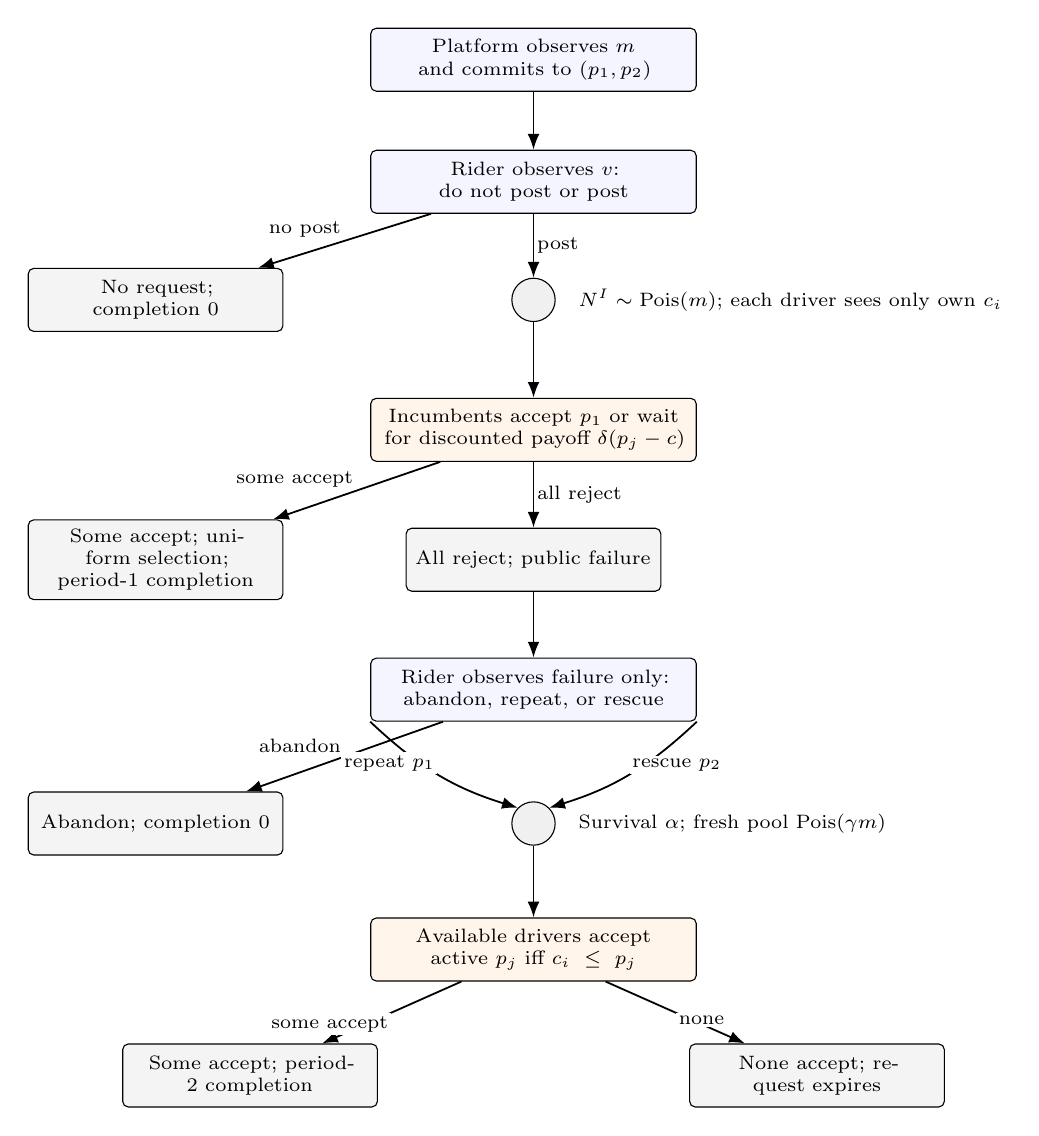
\begin{tikzpicture}[
  x=1cm,y=1cm,>={Latex[length=2mm]},
  flow/.style={->,line width=.65pt},
  box/.style={draw,rounded corners=2pt,align=center,minimum height=8mm,
    text width=39mm,font=\scriptsize,fill=blue!4},
  drv/.style={box,fill=orange!8},
  term/.style={box,fill=gray!9,text width=30mm},
  chance/.style={circle,draw,fill=gray!12,minimum size=5.5mm,inner sep=0pt},
  edge/.style={font=\scriptsize,fill=white,inner sep=1pt}]
\node[box] (platform) at (0,0) {Platform observes $m$ and commits to $(p_1,p_2)$};
\node[box] (rider0) at (0,-1.55) {Rider observes $v$: do not post or post};
\node[term] (nopost) at (-4.8,-3.05) {No request; completion $0$};
\node[chance] (pool) at (0,-3.05) {};
\node[align=left,font=\scriptsize,anchor=west] at (.45,-3.05)
 {$N^I\sim\mathrm{Pois}(m)$; each driver sees only own $c_i$};
\node[drv] (drivers1) at (0,-4.7) {Incumbents accept $p_1$ or wait for discounted payoff $\delta(p_j-c)$};
\node[term] (done1) at (-4.8,-6.35) {Some accept; uniform selection; period-1 completion};
\node[term] (fail) at (0,-6.35) {All reject; public failure};
\node[box] (rider1) at (0,-8.0) {Rider observes failure only: abandon, repeat, or rescue};
\node[term] (abandon) at (-4.8,-9.7) {Abandon; completion $0$};
\node[chance] (supply2) at (0,-9.7) {};
\node[align=left,font=\scriptsize,anchor=west] at (.45,-9.7)
 {Survival $\alpha$; fresh pool $\mathrm{Pois}(\gamma m)$};
\node[drv] (drivers2) at (0,-11.3) {Available drivers accept active $p_j$ iff $c_i\le p_j$};
\node[term] (done2) at (-3.6,-12.9) {Some accept; period-2 completion};
\node[term] (expire) at (3.6,-12.9) {None accept; request expires};
\draw[flow] (platform)--(rider0);
\draw[flow] (rider0)--node[edge,above left]{no post}(nopost);
\draw[flow] (rider0)--node[edge,right]{post}(pool);
\draw[flow] (pool)--(drivers1);
\draw[flow] (drivers1)--node[edge,above left]{some accept}(done1);
\draw[flow] (drivers1)--node[edge,right]{all reject}(fail);
\draw[flow] (fail)--(rider1);
\draw[flow] (rider1)--node[edge,above left]{abandon}(abandon);
\draw[flow] (rider1.south west) to[bend right=13]
 node[edge,above left]{repeat $p_1$}(supply2.north west);
\draw[flow] (rider1.south east) to[bend left=13]
 node[edge,above right]{rescue $p_2$}(supply2.north east);
\draw[flow] (supply2)--(drivers2);
\draw[flow] (drivers2)--node[edge,below left]{some accept}(done2);
\draw[flow] (drivers2)--node[edge,below right]{none}(expire);
\end{tikzpicture}
\caption{Reduced extensive form.  The realized incumbent count, rival costs,
survival, and fresh entry remain latent at the indicated decisions.}
\label{fig:timing}
\end{figure}

\subsection{Equilibrium class, beliefs, and tie-breaking}

We use weak perfect Bayesian equilibrium (WPBE), restricted to anonymous,
symmetric, pure first-period driver cutoffs.  Under cutoff $a$, incumbents
below $a$ accept and those above $a$ wait.  The cutoff type accepts at an
interior or upper cutoff and rejects at the lower cutoff; this affects only a
null cost type.

The rider posts at a zero payoff when $v=p_1$, and does not post below it.
After failure, the following priority rule makes continuation single-valued.
If the maximal continuation payoff is zero, the rider repeats iff
$\beta v-p_1\ge0$ and otherwise abandons.  If repeat and rescue tie at a
strictly positive maximum, the rider chooses rescue.  Terminal drivers accept
at a zero surplus.  These rules matter when repeat has zero coverage: a
positive interval of rider types can then be indifferent between repeat and
abandon.

For $p_1<1$, posting implies the belief
$v\mid\{\text{post}\}\sim U[p_1,1]$.  Since supply is independent of value,
failure leaves this value posterior unchanged.  Poisson splitting determines
the rider's supply posterior after failure.  For a focal incumbent, Palm
conditioning leaves the number of rivals distributed as $\operatorname{Pois}(m)$.
At $(p_1,p_2)=(1,1)$, posting is a null event; we complete the off-path driver
subgame with cutoff one and define completion as zero.

\section{Equilibrium under an arbitrary announced menu}
\label{sec:equilibrium}

Fix a candidate cutoff $a\in[0,p_1]$ and define
\[
 \ph(x)=
 \begin{cases}(1-e^{-x})/x,&x>0,\\1,&x=0,\end{cases}
 \qquad
 \lambda_j(a)=m\{\alpha(p_j-a)+\gamma p_j\},
 \qquad C_j(a)=1-e^{-\lambda_j(a)}.
 \tag{1}
\]

\begin{lemma}[Poisson competition and failure posterior]
\label{lem:poisson}
Under cutoff $a$, first-period completion conditional on posting is
$1-e^{-ma}$.  A focal acceptor's expected assignment share is $\ph(ma)$,
while a focal waiting driver reaches failure against all rivals with
probability $e^{-ma}$.  Conditional on universal rejection, incumbents above
$a$ remain a Poisson marked population.  After survival and fresh entry,
terminal coverage at $p_j$ is $C_j(a)$, and an eligible focal driver's
terminal assignment share is $\ph(\lambda_j(a))$.
\end{lemma}

The assignment identity follows from
\[
 \E\left[\frac1{1+Z}\right]=\int_0^1\E[t^Z]dt
 =\frac{1-e^{-x}}x,\qquad Z\sim\operatorname{Pois}(x).
\]
Poisson marking gives independent counts below and above $a$.  Conditional on
no point below $a$, the above-$a$ process is unchanged.  This is not the law
of $N^I-1$ conditional on $N^I\ge1$.

After failure, rider payoffs from abandon, repeat, and rescue are
\[
 0,\qquad C_1(a)(\beta v-p_1),\qquad
 C_2(a)(\beta v-p_2).
\]
If $C_2>C_1$, define
\[
 v^M(a)=\frac{C_2(a)p_2-C_1(a)p_1}
 {\beta[C_2(a)-C_1(a)]};
\]
if $C_2=C_1$, put $v^M=+\infty$.  Conditional on posting, the repeat and
rescue masses are
\[
 \eta^R(a)=
 \frac{[\min\{v^M(a),1\}-p_1/\beta]^+}{1-p_1},
 \qquad
 \eta(a)=\frac{[1-v^M(a)]^+}{1-p_1},             \tag{2}
\]
and
\[
 \eta^R(a)+\eta(a)=
 \rho(p_1):=\frac{[1-p_1/\beta]^+}{1-p_1}.       \tag{3}
\]
The initial posting payoff is
\[
 (1-e^{-ma})(v-p_1)+e^{-ma}
 \max\{0,C_1(\beta v-p_1),C_2(\beta v-p_2)\},
\]
so the rider posts exactly when $v\ge p_1$.

A focal incumbent of cost $c$ obtains
\[
 A(c;a)=\ph(ma)(p_1-c)                           \tag{4}
\]
from accepting immediately and
\[
 W(c;a)=\delta\alpha e^{-ma}\left\{
 \eta^R(a)\ph(\lambda_1(a))[p_1-c]^+
 +\eta(a)\ph(\lambda_2(a))[p_2-c]^+
 \right\}                                       \tag{5}
\]
from waiting.  These are conditional on observing a posted request; the
posting mass must not multiply a driver's sequential payoff.

For $c\le p_1$, the margin $A-W$ is affine and strictly decreasing in $c$:
\[
 A(c;a)-W(c;a)=B(a)(p_1-c)-D(a),                 \tag{6}
\]
where
\[
\begin{aligned}
 B(a)&=\ph(ma)-\delta\alpha e^{-ma}
 \{\eta^R(a)\ph(\lambda_1)+\eta(a)\ph(\lambda_2)\},\\
 D(a)&=\delta\alpha e^{-ma}\eta(a)\ph(\lambda_2)(p_2-p_1).
\end{aligned}
\]
Indeed, $B(a)>0$ for $p_1>0$ because
\[
 B(a)\ge\ph(ma)-\delta e^{-ma}\ge0,
\]
with strictness from $a>0$ or, at $a=0$, from $\rho(p_1)<1$.  Hence a best
response is genuinely a cutoff.

Define the cutoff-type margin
\[
 f_m(a;p_1,p_2)=\ph(ma)(p_1-a)
 -\delta\alpha e^{-ma}\left\{
 \eta^R(a)\ph(\lambda_1)(p_1-a)
 +\eta(a)\ph(\lambda_2)(p_2-a)
 \right\}.                                      \tag{7}
\]

\begin{proposition}[Symmetric cutoff WPBE]
\label{prop:wpbe}
For $0<p_1<1$, the equilibrium cutoff set is
\[
\begin{aligned}
 \calE_m^{\alpha,\delta,\gamma}(p_1,p_2)
 =&\ \{0:f_m(0;p_1,p_2)\le0\}\\
 &\cup\{a\in(0,p_1):f_m(a;p_1,p_2)=0\}\\
 &\cup\{p_1:f_m(p_1;p_1,p_2)\ge0\}.
\end{aligned}                                    \tag{8}
\]
It is nonempty and compact.  At $p_1=0$, the only aggregate cutoff is zero
with the lower-boundary reject action; at $(1,1)$, set
$\calE_m^{\alpha,\delta,\gamma}(1,1)=\{1\}$.  Thus every feasible menu admits an
anonymous symmetric pure-cutoff WPBE.
\end{proposition}

At the upper boundary,
\[
 f_m(p_1;p_1,p_2)=
 -\delta\alpha e^{-mp_1}\eta(p_1)\ph(\lambda_2(p_1))(p_2-p_1)\le0,
\]
so $a=p_1$ is eligible precisely when the right side is zero.  Continuity of
$f_m$, the lower-boundary test, and the intermediate value theorem give
existence; endpoint limits remain eligible, proving compactness.

For $p_1<1$, completion on cutoff branch $a$ is
\[
 M_m^{\alpha,\gamma}(p_1,p_2;a)
 =(1-p_1)\left[1-e^{-ma}+e^{-ma}
 \{\eta^R(a)C_1(a)+\eta(a)C_2(a)\}\right].       \tag{9}
\]
We define the conservative value within the stated class by
\[
 \underline M_m^{\alpha,\delta,\gamma}(p_1,p_2)
 =\min_{a\in\calE_m^{\alpha,\delta,\gamma}(p_1,p_2)}
 M_m^{\alpha,\gamma}(p_1,p_2;a),                \tag{10}
\]
which is well-defined by Proposition~\ref{prop:wpbe}.  The announced value is
\[
 D_{\alpha,\delta,\gamma}^*(m)
 =\sup_{(p_1,p_2)\in\mathcal P^D}
 \underline M_m^{\alpha,\delta,\gamma}(p_1,p_2). \tag{11}
\]
We retain a supremum here; attainment will be proved for the main no-entry
baseline rather than assumed in the general model.

\section{Flat-payment benchmark}
\label{sec:flat}

\begin{proposition}[Flat policy]
\label{prop:flat}
For every $m>0$ and $p>0$, $(p,p)$ has the unique numeric cutoff $a=p$.
Its completion is
\[
 Q^F_\gamma(m,p)
 =(1-p)(1-e^{-mp})
 +e^{-mp}[1-p/\beta]^+(1-e^{-\gamma mp}).        \tag{12}
\]
Consequently
\[
 F_\gamma^*(m)=\max_{p\in[0,1]}Q^F_\gamma(m,p)  \tag{13}
\]
is attained.
\end{proposition}

For $a<p$, the flat cutoff margin factors as
\[
 (p-a)\left[\ph(ma)-\delta\alpha e^{-ma}\rho(p)
 \ph\bigl(m\{\alpha(p-a)+\gamma p\}\bigr)\right]>0,
\]
so no lower cutoff is sustainable.  At $a=p$, surviving rejectors have cost
above $p$ and do not accept the same payment later; only fresh drivers can
complete after failure, which gives (12).  Continuity on $[0,1]$ gives the
maximum in (13).

\section{Local escalation with fresh entry}
\label{sec:localentry}

The general equilibrium characterization permits a sharp local comparison
even when fresh drivers enter.  Fix $0<p<\beta$ and abbreviate
\[
 x=mp,\quad R=e^{-x},\quad E=e^{-\gamma x},\quad
 \sigma=\ph(x),\quad \ell=\ph(\gamma x),\quad
 \rho=\frac{1-p/\beta}{1-p}.                               \tag{L1}
\]
For $\alpha+\gamma>0$, define the limiting repeat--rescue switch and rescue
mass by
\[
 \bar v=\frac1\beta\left[p+
  \frac{1-E}{mE(\alpha+\gamma)}\right],\qquad
 \eta^0=\frac{1-\bar v}{1-p}.                              \tag{L2}
\]
At $\gamma=0$, the fraction in (L2) is zero.

\begin{theorem}[Fresh-entry local rescue]
\label{thm:localentry}
Suppose $m>0$, $0<p<\beta<1$, $0<\delta\le1$,
$0\le\alpha\le1$, $\gamma\ge0$,
$\alpha+\gamma>0$, and $\bar v<1$.  For all sufficiently small
$\varepsilon>0$, the menu $(p,p+\varepsilon)$ has a unique anonymous
symmetric cutoff WPBE, with
\[
 a_\varepsilon=p-\kappa\varepsilon+o(\varepsilon),\qquad
 \kappa=\frac{\delta R\alpha\ell\eta^0}
 {\sigma-\delta R\alpha\rho\ell}.                       \tag{L3}
\]
Every candidate cutoff is uniformly localized by
\[
 0\le p-a_\varepsilon
 \le\frac{\delta\alpha\rho}{1-\delta\alpha\rho}
 \varepsilon.                                                \tag{L4}
\]
The right derivative of completion is
\[
 \left.\frac{dM_m^{\alpha,\gamma}(p,p+\varepsilon;
 a_\varepsilon)}{d\varepsilon}\right|_{0+}
 =m(1-p)R\eta^0
 \frac{T_\delta}{\sigma-\delta R\alpha\rho\ell}>0,       \tag{L5}
\]
where
\[
 T_\delta=E(\alpha+\gamma)\sigma
 -\delta R\alpha\ell\{1-\rho+\rho E(1+\gamma)\}>0.       \tag{L6}
\]
\end{theorem}

The activity condition $\bar v<1$ says that a positive mass of riders uses
marginal rescue after failure.  It is automatic at $\gamma=0$ but substantive
with entry.  The knife edge $\bar v=1$ needs a second-order rider-mass
expansion and is not included.  For $\gamma>1$, activity cannot simply be
deleted from the sign claim: for example
\[
 x=1,\quad p=\tfrac12,\quad m=2,\quad \beta=\tfrac{51}{100},
 \quad\alpha=1,\quad\gamma=10,\quad\delta=\tfrac12
\]
has $\bar v>1$ and makes $T_\delta$ in (L6) negative.  Thus the
theorem's restriction is economically and mathematically real.

\section{Global menu design without fresh entry}
\label{sec:global}

We now solve the primary baseline
\[
 \gamma=0,\qquad m>0,\qquad \alpha\in(0,1],\qquad
 \beta\in(0,1),\qquad \delta\in(0,1].
\]
Write $(p,q)=(p_1,p_2)$ and $k=\alpha m$.  Menus with $p\ge\beta$ or
$q\ge\beta$ cannot induce positive-mass rescue and are outcome-equivalent to
the flat first payment.  The nontrivial region is therefore
$0\le p<q<\beta$.

For $a\in[0,p]$, put
\[
 C(x)=1-e^{-kx},\qquad
 h(a)=\begin{cases}(e^{ma}-1)/a,&a>0,\\m,&a=0,\end{cases}   \tag{14}
\]
and
\[
 A_z(a)=(\beta-z)C(z-a),\quad z\in\{p,q\},
 \qquad B_p=\beta(1-p).                                    \tag{15}
\]
The repeat--rescue switch lies below one exactly when $A_q(a)>A_p(a)$.
Substitution of the switch type into continuation coverage gives the exact
cancellation
\[
 K_{p,q}(a)
 =\frac{\max\{A_p(a),A_q(a)\}}{B_p}.                       \tag{16}
\]
Multiplying the cutoff driver's payoff margin by the positive factor
$me^{ma}$ gives the sign-equivalent scalar
\[
 \mathcal D_{p,q}^{\delta}(a)
 =(p-a)h(a)-\delta K_{p,q}(a).                             \tag{17}
\]

The repeat branch cannot contain a cutoff below $p$:
\[
 (p-a)h(a)>\frac{A_p(a)}{B_p}
 \ge\delta\frac{A_p(a)}{B_p},\qquad 0\le a<p.              \tag{18}
\]
For $a>0$, this is $\ph(ma)>e^{-ma}$ combined with
$\alpha\rho\ph(k(p-a))\le1$; at $a=0$, strictness follows from
$\rho(p)<1$.  Hence every zero of (17) under a strict active menu lies on the
rescue branch, not at the rider kink.

\begin{theorem}[Global cutoff uniqueness]
\label{thm:unique}
Fix $0\le p<q<\beta$.  If $\mathcal D_{p,q}^{\delta}(0)\le0$, the unique numeric
cutoff is the lower-boundary cutoff $a=0$.  If
$\mathcal D_{p,q}^{\delta}(0)>0$, there is a unique cutoff $a\in(0,p)$.  Equality at
zero never coexists with a positive root.  Together with the flat,
repeat-only, $p=0$, and $\alpha=0$ boundary cases, every no-entry menu has a
unique numeric symmetric cutoff under the stated cutoff-type convention.
\end{theorem}

The one-crossing argument is global.  At an active-rescue zero write
$u=p-a$, $z=q-a$, $b=\beta-q$, and $B=\beta(1-p)$.  The root equation is
\[
 uh(a)=\delta\frac bB C(z).
\]
Since $B-b=q-\beta p>0$ and $h(a)\ge m$, $u<C(z)/m$.  For
$R(a)=u h(a)/C(z)$,
\[
 \frac{R'(a)}{R(a)}
 =-\frac1u+\frac{h'(a)}{h(a)}+\frac{k}{e^{kz}-1}<0,          \tag{19}
\]
because
\[
 \frac1u-\frac{k}{e^{kz}-1}
 >m\frac{1-\alpha e^{-kz}}{1-e^{-kz}}
 \ge m>\frac{h'(a)}{h(a)}.
\]
Thus every zero crosses downward.  Since
$\mathcal D_{p,q}^{\delta}(p)<0$, two zeros would require an intervening upward
crossing.  At $p=0$, the numeric cutoff is zero and the cost-zero type uses
the lower-boundary reject action.

\subsection{Completion identity and comparison with the same flat payment}

At any positive cutoff, indifference gives
\[
 e^{-ma}K_{p,q}(a)=\frac{m\ph(ma)(p-a)}\delta.
\]
Using $1-e^{-ma}=ma\ph(ma)$ in (9) yields
\[
 \boxed{M_m^{\alpha,\delta,0}(p,q;a)
 =(1-p)m\ph(ma)\left[a+\frac{p-a}\delta\right],
 \qquad a>0.}                                               \tag{20}
\]
At a reject-all equilibrium,
\[
 M_m^{\alpha,\delta,0}(p,q;0)=
 \left(1-\frac q\beta\right)(1-e^{-kq})
 \ge\frac{(1-p)mp}{\delta},                                \tag{21}
\]
with equality exactly at the lower-boundary indifference condition.  Repeat
may be used by positive mass in (21); its contribution cancels algebraically.

Both $\ph(ma)$ and $a+(p-a)/\delta$ weakly decrease in $a>0$, and the
first decreases strictly, so (20) decreases with the cutoff.
Theorem~\ref{thm:unique} then gives a particularly strong comparison.  For
every $0<p<q<\beta$, the strict-menu cutoff is below $p$, and therefore
\[
 \underline M_m^{\alpha,\delta,0}(p,q)>F_m(p)
 =(1-p)(1-e^{-mp}).                                         \tag{22}
\]
This is a global same-$p$ result, not merely a derivative along one selected
branch.

For completeness, a one-sided local expansion at $(p,p)$ is
\[
 a_\varepsilon=p-\kappa\varepsilon+o(\varepsilon),
 \qquad
 \kappa=
 \frac{\delta e^{-mp}\alpha\rho}
 {\ph(mp)-\delta e^{-mp}\alpha\rho},                       \tag{23}
\]
and
\[
 \left.\frac{dM(p,p+\varepsilon)}{d\varepsilon}\right|_{0+}
 =\frac{m(1-p)e^{-mp}\alpha\rho
 [\ph(mp)-\delta e^{-mp}]}
 {\ph(mp)-\delta e^{-mp}\alpha\rho}>0.                    \tag{24}
\]
The wedge decomposes as
$\ph(mp)-\delta e^{-mp}=[\ph(mp)-e^{-mp}]+(1-\delta)e^{-mp}$:
assignment competition is the first term and incumbent impatience the second.

\subsection{The fixed-first-payment problem}

Following the design sequence, fix $p$ before optimizing $q$.  For a target
cutoff $a<\beta$, maximize
\[
 A(a,q)=(\beta-q)[1-e^{-k(q-a)}],\qquad q\in[a,\beta].       \tag{25}
\]
It is strictly concave.  Its unique maximizer $Q(a)$ satisfies
\[
 e^{k(Q(a)-a)}-1=k(\beta-Q(a)),                              \tag{26}
\]
or
\[
 Q(a)=\beta-
 \frac{W_0(e^{1+k(\beta-a)})-1}{k}.                         \tag{27}
\]
Moreover
\[
 a<Q(a)<\frac{a+\beta}{2}.
\]
Let
\[
 S(a)=A(a,Q(a)),\qquad
 S(a)=\frac{k[\beta-Q(a)]^2}{1+k[\beta-Q(a)]}.              \tag{28}
\]
Define $Q_0=Q(0)$, $S_0=S(0)$, and
\[
 p_z=\frac{1-\sqrt{1-4\delta S_0/(\beta m)}}2.             \tag{29}
\]
The strict flat inequality at $p=Q_0,a=0$ gives
$0<p_z<Q_0<1/2$.

\begin{theorem}[Optimal rescue conditional on the first payment]
\label{thm:fixedp}
Let
\[
 H_m(p)=\max_{q\in[p,1]}\underline M_m^{\alpha,\delta,0}(p,q).
\]
Then:
\begin{enumerate}[label=(\roman*)]
 \item If $0\le p\le p_z$, the unique optimal rescue is $q=Q_0$, the
 cutoff is the lower-boundary reject-all cutoff $a=0$, and
 \[
 H_m(p)=S_0/\beta.
 \]
 \item If $p_z<p<\beta$, there is a unique $a^*(p)\in(0,p)$ satisfying
 \[
 (p-a)h(a)=\frac{\delta S(a)}{\beta(1-p)}.                  \tag{30}
 \]
 The unique optimal rescue is $q=Q(a^*(p))$, and
 \[
 H_m(p)=(1-p)m\ph(ma^*(p))
 \left[a^*(p)+\frac{p-a^*(p)}\delta\right].
 \]
 \item If $\beta\le p\le1$, every $q\in[p,1]$ is outcome-equivalent and
 \[
 H_m(p)=(1-p)(1-e^{-mp}).
 \]
\end{enumerate}
Thus the conditional supremum is a maximum in every regime.
\end{theorem}

To see implementability, a positive target cutoff solves
\[
 A(a,q)=\frac{\beta(1-p)(p-a)h(a)}\delta.                  \tag{31}
\]
The right side strictly exceeds $A(a,p)$ by (18), so (31) cannot generate a
repeat-only or kink pseudo-solution.  If the envelope is below, equal to, or
above the right side, there are respectively zero, one tangent, or two strict
implementing prices.  Theorem~\ref{thm:unique} makes each implemented cutoff
the unique equilibrium.  Completion falls with the cutoff, so the smallest
implementable cutoff, attained at tangency, solves the fixed-$p$ problem.

\subsection{One-dimensional global design and attainment}

Define
\[
 R_\delta(a)=\frac{\delta S(a)}{\beta h(a)}.
\]
The tangent equation is
\[
 (1-p)(p-a)=R_\delta(a).                                     \tag{32}
\]
Because $Q(a)<(1+a)/2$ and the left side is increasing in $p$ below that
vertex, the unique feasible root is the lower quadratic branch
\[
 \boxed{
 P_\delta(a)=
 \frac{1+a-\sqrt{(1-a)^2-4R_\delta(a)}}2.}                 \tag{33}
\]
The upper branch is not a fixed-$p$ rescue optimum.  The map $P_\delta$ is
continuous and strictly increasing from $[0,\beta]$ onto $[p_z,\beta]$.
Endpoint injectivity follows from the same envelope one-crossing argument:
$P_\delta(a)=P_\delta(0)=p_z$ for $a>0$ would give the fixed-$p_z$
envelope two zeros.

Extend $P_\delta(\beta)=Q(\beta)=\beta$ and set
\[
 J_\delta(a)=
 \begin{cases}
 (1-P_\delta(a))m\ph(ma)
 \left[a+\dfrac{P_\delta(a)-a}\delta\right],&a>0,\\[6pt]
 mp_z(1-p_z)/\delta=S_0/\beta,&a=0.
 \end{cases}                                                \tag{34}
\]
Then $J_\delta(\beta)=(1-\beta)(1-e^{-m\beta})$, and the complete outer
problem is
\[
 \boxed{
 D_{\alpha,\delta,0}^*(m)=
 \max\left\{
 \max_{a\in[0,\beta]}J_\delta(a),
 \max_{p\in[\beta,1]}(1-p)(1-e^{-mp})
 \right\}.}                                                 \tag{35}
\]

\begin{theorem}[Policy attainment and optimized-flat dominance]
\label{thm:global}
For every no-entry parameter tuple with $m>0$ and $\alpha>0$, the announced
policy value in (11) is attained.  If $\beta\ge1/2$, every optimal menu is a
strict menu
\[
 (p_1^*,p_2^*)=(P_\delta(a^*),Q(a^*)),
 \qquad a^*\in\argmax_{a\in[0,\beta]}J_\delta(a)
 \subset(0,\beta),                                          \tag{36}
\]
and
\[
 D_{\alpha,\delta,0}^*(m)>F_0^*(m).                         \tag{37}
\]
No uniqueness of $a^*$ is asserted.
\end{theorem}

Equation (35) is a maximum of continuous functions on compact intervals, so
it proves attainment directly.  In the no-entry flat problem,
\[
 F_m(p)=(1-p)(1-e^{-mp})
\]
is strictly concave and its unique optimizer is
\[
 p_F(m)=\frac{1+m-W_0(e^{1+m})}{m}<\frac12.                 \tag{38}
\]
For $\beta\ge1/2$, $p_F<\beta$, and (22) applied at $p_F$ proves (37),
including the equality case $\beta=1/2$.  The boundary portions of (35) do
not beat $F_0^*$, whereas (37) does, so every global optimizer is interior and
strict.

The driver discount also yields a clean comparative static.  Write
$R_1(a)=S(a)/[\beta h(a)]$, so that
$(1-P_\delta)(P_\delta-a)=\delta R_1(a)$.  For
$a\in(0,\beta)$,
\[
 \frac{\partial P_\delta(a)}{\partial\delta}
 =\frac{R_1(a)}{1+a-2P_\delta(a)}>0,
 \qquad
 \frac{\partial J_\delta(a)}{\partial\delta}
 =-(1-e^{-ma})
 \frac{\partial P_\delta(a)}{\partial\delta}<0.            \tag{38a}
\]
Thus $D_{\alpha,\delta,0}^*(m)$ is weakly decreasing in $\delta$: more
patient incumbents require a higher first payment to implement the same
cutoff and continuation coverage.  This is a completion comparative static,
not a welfare ranking.

\subsection{The full patience region}

Fix $(m,\alpha,\delta)$ and make patience explicit in $D(m;\beta)$.  For a fixed
strict menu $p<q$, its value equals $F_m(p)$ for $\beta\le q$ and is strictly
increasing for $\beta>q$.  Indeed, increasing $\beta$ raises the active-rescue
coefficient in (17), shifts the unique cutoff strictly left (or to zero), and
then raises completion by (20)--(21).

The scalar representation is jointly continuous in patience.  To use a fixed
choice set, write $a=\beta x$.  The solution of
\[
 e^{ky}-1=k\{\beta(1-x)-y\}
\]
is continuous in $(\beta,x)$.  At $x=0$, $h(0)=m$ and
$P_{\beta,\delta}(0)=p_z(\beta)$ has a strictly positive discriminant; at
$x=1$, $P_{\beta,\delta}(\beta)=Q_\beta(\beta)=\beta$ and
$J_{\beta,\delta}(\beta)=(1-\beta)(1-e^{-m\beta})$.  These removable extensions and
the elementary maximum theorem make $D(m;\beta)$ continuous.

Define
\[
 \beta_c(m,\alpha,\delta)=
 \inf\{\beta\in(0,1):D_{\alpha,\delta,0}^*(m;\beta)>F_0^*(m)\}. \tag{39}
\]

\begin{theorem}[Patience threshold]
\label{thm:patience}
For $m>0$, $0<\alpha\le1$, and $0<\delta\le1$, the strict-gain region is the single upper
interval
\[
 D_{\alpha,\delta,0}^*(m;\beta)>F_0^*(m)
 \quad\Longleftrightarrow\quad
 \beta>\beta_c(m,\alpha,\delta).                           \tag{40}
\]
Moreover
\[
 0< -\frac1m\log(1-F_0^*(m))
 \le\beta_c(m,\alpha,\delta)\le p_F(m)<\frac12.           \tag{41}
\]
For fixed $(m,\alpha,\delta)$, $D(m;\beta)=F_0^*(m)$ through the threshold and is
strictly increasing above it.  The exact scalar test is
\[
 \beta>\beta_c(m,\alpha,\delta)
 \quad\Longleftrightarrow\quad
 \max_{a\in[0,\beta]}J_{\beta,\delta}(a)>F_0^*(m).        \tag{42}
\]
When $\alpha=0$, the gain region is empty.
\end{theorem}

Pointwise monotonicity in (38a) also nests the thresholds:
\[
 0<\delta_1<\delta_2\le1
 \quad\Longrightarrow\quad
 \beta_c(m,\alpha,\delta_1)
 \le\beta_c(m,\alpha,\delta_2).                            \tag{42a}
\]
Strict inequality is not asserted globally.

The lower bound follows because an active menu has $q<\beta$ and completion
requires an initial incumbent with cost at most $q$, giving
$M<1-e^{-m\beta}$.  The upper bound follows from a strict menu at $p_F$ when
$\beta>p_F$.  If gain holds at one patience level, attainment supplies an
optimal strict menu; reusing it at any larger $\beta$ and applying the fixed
menu monotonicity gives strict gain and strict value increase.  Continuity
makes the gain interval open.

\section{Market thickness: topology and endpoint rates}
\label{sec:thickness}

Fix $0<\alpha\le1$, $0<\beta<1$, $0<\delta\le1$, and $\gamma=0$.  Define
the optimized value of commitment by
\[
 V_{\alpha,\delta,0}(m)
 =D_{\alpha,\delta,0}^*(m)-F_0^*(m).                       \tag{43}
\]
The outer representation (35), rather than a local-menu derivative, is the
appropriate object because the optimal menu moves with thickness.

For the thin limit, define on $a\in[0,\beta]$
\[
 P_0^\delta(a)=
 \frac{1+a-\sqrt{(1-a)^2-
 \delta\alpha(\beta-a)^2/\beta}}2,
 \qquad
 H_0^\delta(a)=a[1-P_0^\delta(a)]
 +\frac{\alpha(\beta-a)^2}{4\beta},                       \tag{44}
\]
and $G_{\alpha,\beta,\delta}=\max_{a\in[0,\beta]}H_0^\delta(a)$.

\begin{theorem}[Thickness topology and exact endpoint regimes]
\label{thm:thickness}
For fixed $(\alpha,\beta,\delta)\in(0,1]\times(0,1)\times(0,1]$:
\begin{enumerate}[label=(\roman*)]
 \item $D_{\alpha,\delta,0}^*(m)$, $F_0^*(m)$, and
 $V_{\alpha,\delta,0}(m)$ are continuous on $(0,\infty)$.  The scalar
 cutoff and flat-price argmax correspondences are nonempty, compact valued,
 and upper hemicontinuous.

 \item If $\beta>1/2$ and $\delta<1$, then
 \[
  V_{\alpha,\delta,0}(m)
  \sim\left(G_{\alpha,\beta,\delta}-\frac14\right)m,
  \qquad G_{\alpha,\beta,\delta}>\frac14.                 \tag{45}
 \]
 At the no-discount boundary $\delta=1$, let $a_0\in(0,1/2)$ be the
 unique solution of
 \[
  \alpha(\beta-a_0)^2=\beta(1-2a_0).
 \]
 Then
 \[
  V_{\alpha,1,0}(m)\sim\frac{1-2a_0}{16}m^2.              \tag{46}
 \]

 \item If $\beta=1/2$ and $\delta<1$, then
 \[
  V_{\alpha,\delta,0}(m)
  \sim
  \frac{\alpha(1-\delta)}
  {512\{1-\alpha(1-\delta)/2\}}m^3.                       \tag{47}
 \]
 At $\delta=1$, the leading cancellation persists one order longer:
 \[
  V_{\alpha,1,0}(m)\sim\frac{\alpha}{2048}m^4.            \tag{48}
 \]

 \item If $\beta<1/2$, there exists
 $m_0(\alpha,\beta,\delta)>0$ such that
 \[
  D_{\alpha,\delta,0}^*(m)=F_0^*(m),\qquad
  V_{\alpha,\delta,0}(m)=0,
  \qquad 0<m<m_0(\alpha,\beta,\delta).                   \tag{49}
 \]

 \item As $m\to\infty$,
 \[
  1-D_{\alpha,\delta,0}^*(m)\sim\frac{\log\log m}{m},
  \quad 1-F_0^*(m)\sim\frac{\log m}{m},
  \quad V_{\alpha,\delta,0}(m)\sim\frac{\log m}{m}.     \tag{50}
 \]
 For each fixed positive $(\alpha,\beta)$, the estimates establishing (50)
 are uniform over the full policy/cutoff domain and uniformly over
 $\delta\in(0,1]$.  They are not uniform over primitive sequences with
 $\alpha\downarrow0$ or $\beta\downarrow0$.
\end{enumerate}
\end{theorem}

Equations (45)--(48) show a singular boundary: the limits $m\downarrow0$ and
$\delta\uparrow1$ do not commute at the first nonzero order.  Even slight
incumbent impatience creates a first-order screening gain when $\beta>1/2$
and a cubic gain at $\beta=1/2$; exact patience removes those terms.

Here is the proof architecture.  Let $k=\alpha m$ and let $z_m(a)$ solve
\[
 z_m(a)+\log[1+z_m(a)]=k(\beta-a),
 \qquad y_m(a)=z_m(a)/k.
\]
Then
\[
 Q_m(a)=\beta-y_m(a),\quad
 T_m(a)=\frac{k y_m(a)^2}{\beta[1+k y_m(a)]},\quad
 B_m^\delta(a)=\delta\frac{a}{e^{ma}-1}T_m(a),             \tag{51}
\]
with $a/(e^{ma}-1)=1/m$ at zero, and
\[
 P_m^\delta(a)=
 \frac{1+a-\sqrt{(1-a)^2-4B_m^\delta(a)}}2.               \tag{52}
\]
The scalar objective admits the useful exact form
\[
 J_m^\delta(a)
 =[1-P_m^\delta(a)](1-e^{-ma})+T_m(a)e^{-ma}.              \tag{53}
\]
The strict envelope bound keeps the discriminant positive.  Joint
continuity and Berge's maximum theorem prove part (i).

Uniformly on $[0,\beta]$, $P_m^\delta\to P_0^\delta$ and
$J_m^\delta/m\to H_0^\delta$.  If $\beta>1/2$ and $\delta<1$, the unique
$a\in(0,1/2)$ satisfying $P_0^\delta(a)=1/2$ gives
\[
 H_0^\delta(a)=\frac12\left[a+\frac{1/2-a}{\delta}\right]
 >\frac14,
\]
which proves the strict coefficient in (45); uniform convergence gives its
exact value as the maximum in (44).  For $\delta=1$, the first-order term
ties the flat benchmark, and the uniform second-order argmax expansion gives
(46).

At $\beta=1/2$, every thin optimizer localizes as $a=1/2-cm$.  Put
$A_\delta=1-\alpha(1-\delta)/2$.  Uniformly for bounded $c$,
\[
 J_m^\delta(1/2-cm)
 =\frac m4-\frac{m^2}{16}
 +m^3\left\{\frac1{96}+\frac c8-A_\delta c^2\right\}
 +O(m^4).                                                   \tag{54}
\]
The maximizing rescaled cutoff is $c^*=1/(16A_\delta)$, while the flat
$m^3$ coefficient is $11/768$.  Their difference is exactly the coefficient
in (47).  When $\delta=1$ it vanishes; the fourth-order expansion yields
(48).  In particular, uniformly for bounded $c$,
\[
 \begin{aligned}
 J_m^1(1/2-cm)
 &=\frac m4-\frac{m^2}{16}+m^3 f_2(c)+m^4 f_3(c)+o(m^4),\\
 f_2(c)&=\frac{11}{768}-\left(c-\frac1{16}\right)^2,\\
 f_3(c)&=-\frac1{768}-\frac c{24}+\frac{c^2}{4}+2\alpha c^3,
 \end{aligned}                                             \tag{54a}
\]
whereas
\[
 F_0^*(m)=\frac m4-\frac{m^2}{16}
 +\frac{11}{768}m^3-\frac3{1024}m^4+o(m^4).              \tag{54b}
\]
The strict quadratic loss in $f_2$ and local Lipschitz control of $f_3$
evaluate the perturbed maximum at $c=1/16$ to fourth order, and
$f_3(1/16)=-3/1024+\alpha/2048$.  Subtracting (54b) proves (48).
If $\beta<1/2$, the bound
\[
 H_0^\delta(a)
 \le a(1-a)+\frac{(\beta-a)^2}{4\beta}
 \le\beta(1-\beta)<\frac14
\]
is uniform on $[0,\beta]$.  Since the flat optimizer converges to $1/2$,
the flat policy wins exactly on a nonempty initial interval, proving (49).

For the thick limit put $x=ma$, $p=P_m^\delta(a)$, and $T=T_m(a)$.  Equation
(53) gives the same exact nonnegative loss decomposition for every fixed
$\delta>0$:
\[
 \boxed{1-J_m^\delta(a)=p(1-e^{-x})+(1-T)e^{-x}.}           \tag{55}
\]
The feasible choice $x=\log\log m$ and the policy-uniform lower bound obtained
by splitting at $Q_m(a)=\beta/2$ give the first rate in (50).  The exact flat
first-order condition gives the second, and subtraction gives the third.

\begin{corollary}[A best finite thickness, without a shape theorem]
\label{cor:bestm}
For every fixed positive $(\alpha,\beta,\delta)$ in the maintained ranges,
there exists $m^*\in(0,\infty)$ such that
\[
 V_{\alpha,\delta,0}(m^*)
 =\max_{m>0}V_{\alpha,\delta,0}(m)>0.                      \tag{56}
\]
Strict single-peakedness is false when $\beta<1/2$ because of (49).  For
$\beta\ge1/2$, strict single-peakedness remains open for every fixed
$\delta\in(0,1]$.
\end{corollary}

Continuity, endpoint vanishing, and eventual positivity in (50) localize a
global maximizer to a compact subinterval.  No uniqueness of $m^*$ is claimed.

\section{A public-supply benchmark}
\label{sec:publicN}

The Poisson model makes realized local supply latent.  To separate that
information friction from assignment competition, fix instead a deterministic
incumbent count $n\ge1$ observed by every agent.  We evaluate one announced
menu conditional on that fixed $n$; the exercise removes rival-count
uncertainty without introducing state-contingent pricing.  Keep the timing,
uniform private costs, survival, and no-entry assumption.
For a conjectured cutoff $a$, a focal acceptor faces
$X\sim\operatorname{Bin}(n-1,a)$ accepting rivals, so her assignment share is
\[
 s_n(a):=\E\!\left[\frac1{1+X}\right]
 =\frac{1-(1-a)^n}{na},
 \qquad s_n(0)=1.                                           \tag{57}
\]
Universal rejection occurs against all of her rivals with probability
$(1-a)^{n-1}$.  Conditional on that event, each rival has cost uniform on
$(a,1)$.  If terminal payment $p_j$ is selected, a rival is both surviving
and eligible with probability
\[
 \theta_j(a)=\frac{\alpha(p_j-a)}{1-a};
\]
hence a terminal acceptor's assignment share is $s_n(\theta_j)$ and terminal
coverage is
\[
 C_{j,n}(a)=1-[1-\theta_j(a)]^n
           =n\theta_j(a)s_n(\theta_j(a)).                   \tag{58}
\]

Let $\eta_j(a)$ be the posting-conditional mass of riders who select terminal
payment $p_j$ after failure.  At a positive interior cutoff, indifference of
the cutoff driver is
\[
 s_n(a)(p_1-a)
 =\delta(1-a)^{n-1}\alpha
   \sum_j\eta_j(a)s_n(\theta_j(a))(p_j-a).                  \tag{59}
\]
Substitution of (58)--(59) into unconditional completion gives the exact
finite-population counterpart of (20):
\[
 \boxed{M_n(p_1,p_2;a)
 =(1-p_1)n s_n(a)\left[a+\frac{p_1-a}\delta\right].}       \tag{60}
\]

\begin{proposition}[Public $n$ and local announced rescue]
\label{prop:publicN}
Fix $n\ge1$, $0<\alpha\le1$, $0<\delta\le1$, and
$p\in(0,\beta)$.  For every sufficiently
small $\varepsilon>0$, the menu $(p,p+\varepsilon)$ has a unique symmetric
cutoff, and it satisfies
\[
 a_\varepsilon=p-\kappa_n\varepsilon+o(\varepsilon),
 \qquad
 \kappa_n=
 \frac{\delta(1-p)^{n-1}\alpha\rho(p)}
 {s_n(p)-\delta(1-p)^{n-1}\alpha\rho(p)}>0.                \tag{61}
\]
Its right derivative of unconditional completion is
\[
 \left.\frac{dM_n}{d\varepsilon}\right|_{0+}
 =(1-p)n\kappa_n
 \left\{\frac{1-\delta}{\delta}s_n(p)-p\,s_n'(p)\right\}. \tag{62}
\]
This derivative is strictly positive for every $n\ge1$ when $\delta<1$.
At $\delta=1$, it is strictly positive for $n\ge2$ and exactly zero for
$n=1$.
\end{proposition}

The denominator in (61) is positive because
$s_n(p)\ge(1-p)^{n-1}$ and $\delta\alpha\rho(p)<1$.  Moreover
\[
 s_n(a)=\frac1n\sum_{r=0}^{n-1}(1-a)^r,
\]
which is strictly decreasing for $n\ge2$ and constant for $n=1$.
Proposition~\ref{prop:publicN} rules out the claim that an unobserved realized
count is necessary for the rescue gain.  The first term in (62) is pure
intertemporal compensation and survives at $n=1$; the second is assignment
competition and is positive exactly when $n\ge2$.  Latent supply changes
posterior inference and the global policy problem, but neither local wedge.
If $\alpha=0$, then $\kappa_n=0$ and the derivative in (62) is zero for
every $n$.

\section{Managerial interpretation and institutional scope}
\label{sec:discussion}

The rescue payment is valuable because it is a commitment, not because a
platform can mechanically raise pay after observing failure.  Announcing the
second payment before drivers act makes delay incentive compatible with the
policy and therefore forces the platform to price the delay externality.  In
the no-entry model, the exact fixed-$p_1$ solution says more than ``raise the
payment a little.''  Low first payments optimally generate reject-all and use
the unique rescue-envelope maximizer; intermediate first payments use the
unique tangent rescue that implements the smallest feasible cutoff; once the
first payment reaches rider patience $\beta$, rescue is irrelevant.

Three operational implications follow.  First, the relevant demand-side
state is rider patience, not only nominal willingness to pay.  The exact
threshold $\beta_c(m,\alpha,\delta)$ identifies when commitment beats the best flat
payment, while the simple condition $\beta\ge1/2$ guarantees gain at every
finite thickness.  Second, market thickness changes the form of the optimal
policy.  In a very thick market the dynamic policy closes the request with
loss of order $\log\log m/m$, compared with $\log m/m$ under the best flat
payment.  Yet the absolute difference still vanishes, so a large percentage
reduction in the small residual failure probability should not be confused
with a large unconditional completion gain.  Third, publishing realized
local supply is not enough to eliminate the local mechanism.  Driver
impatience already makes rescue productive with one publicly known incumbent;
assignment competition adds a second gain when there are two or more.

The maintained transfer is paid by the rider to the selected driver, and the
objective is completion.  This maps most directly to bidding, tipping,
top-up, freight, and task platforms.  A platform-funded bonus, profit
maximization, or a bonus budget introduces a real resource cost and is not
covered by the completion theorem.  Likewise, simultaneous acceptance with
uniform selection is a reduced form for a broadcast response window; a
first-response race would add endogenous response effort and is not claimed
to be equivalent.

The equilibrium scope also matters.  The arbitrary-menu analysis covers
anonymous symmetric pure-cutoff WPBE and takes a conservative minimum only
inside that class.  We do not claim robustness to asymmetric or mixed WPBE.
Fresh entry is fully incorporated in the equilibrium characterization and
flat benchmark, but the global menu solution is for $\gamma=0$.  Finally,
the thickness theorem proves existence, endpoint rates, and one exact
failure of strict single-peakedness; it does not prove a unique best
thickness when $\beta\ge1/2$.

\section{Conclusion}
\label{sec:conclusion}

An announced rescue payment changes both continuation coverage and current
acceptance.  Solving those effects jointly reveals a tractable global design
problem.  In the no-entry baseline, every menu has a unique cutoff, the
conditional rescue problem is a concave envelope, and the full two-price
problem reduces to one continuous scalar maximum.  Commitment strictly
beats the optimized flat payment above an endogenous patience threshold and
always does so at $\beta\ge1/2$.  Optimized thickness effects have distinct
thin-market regimes and matching thick-market rates, while strict
single-peakedness is either false or still unproved.  The public-$n$
benchmark decomposes the local gain into intertemporal compensation and
assignment competition, assigning latent supply the narrower role of shaping
inference and global design.

\appendix
\section{Proofs for the equilibrium characterization}
\label{app:equilibrium}

\begin{proof}[Proof of Lemma~\ref{lem:poisson}]
Poisson marking splits the incumbent process into costs below and above $a$,
with independent counts of means $ma$ and $m(1-a)$.  Thus first-period
coverage is $1-e^{-ma}$.  Under Palm conditioning a focal driver's accepting
rivals form a Poisson random variable $Z$ of mean $ma$, and
\[
 \E\!\left[(1+Z)^{-1}\right]
 =\int_0^1\E[t^Z]dt
 =\int_0^1e^{-ma(1-t)}dt=\ph(ma).
\]
If the focal driver waits, continuation is reached only if every rival has
cost above $a$, an event of probability $e^{-ma}$.  Conditional on no point
below $a$, the above-$a$ Poisson process is unchanged.  Independent survival
thins its eligible interval $(a,p_j]$ to intensity
$m\alpha(p_j-a)$, while fresh eligible drivers contribute $m\gamma p_j$.
Superposition gives $\lambda_j$ in (1), terminal coverage $C_j$, and the
same integral identity gives terminal assignment share $\ph(\lambda_j)$.
\end{proof}

\begin{proof}[Proof of Proposition~\ref{prop:wpbe}]
Given a posted request, failure is independent of $v$, so the rider retains
the posterior $U[p_1,1]$.  Comparing the two affine continuation payoffs
gives $v^M$ and the masses in (2); the stated priority rule assigns the
zero-payoff and positive repeat--rescue ties.  Before posting, a type
$v<p_1$ has strictly negative payoff from immediate completion and cannot
obtain positive delayed surplus because $\beta v-p_j<v-p_1<0$.  A type
$v\ge p_1$ obtains a nonnegative immediate payoff whenever a driver accepts
and otherwise can abandon.  The posting rule therefore is exactly
$v\ge p_1$.

For $c\le p_1$, equations (4)--(5) give the affine margin (6).  Since
$\eta^R+\eta=\rho(p_1)<1$ whenever it is positive,
\[
 B(a)\ge\ph(ma)-\delta e^{-ma}
 \ge\ph(ma)-e^{-ma}>0\quad(a>0),
\]
and at $a=0$,
$B(0)\ge1-\delta\alpha\rho(p_1)>0$.  Thus $A-W$ is strictly decreasing in cost;
types above $p_1$ never prefer the negative current surplus to waiting.  A
symmetric best response is consequently a genuine cutoff, and evaluation at
its cutoff type gives (7).

At $a=p_1$, $f_m(p_1)\le0$.  If $f_m(0)\le0$, the lower boundary is an
equilibrium.  If $f_m(0)>0$ and $f_m(p_1)<0$, continuity and the intermediate
value theorem give an interior zero; if $f_m(p_1)=0$, the upper boundary is
an equilibrium.  The aggregate continuation payoff is continuous across a
rider switch because tied actions have equal coverage-weighted utility;
when all continuation coverage is zero the driver's wait payoff is zero.
Hence $f_m$ is continuous.  The same argument shows that any convergent
sequence of eligible boundary points or zeros has an eligible limit, so the
nonempty equilibrium set is closed in $[0,p_1]$ and therefore compact.
The separately stated $p_1=0$ and $(1,1)$ conventions close the remaining
endpoints.  Formula (9) is continuous on the compact equilibrium set, making
the minimum in (10) well defined.
\end{proof}

\begin{proof}[Proof of Proposition~\ref{prop:flat}]
For $a<p$, the cutoff margin is $(p-a)$ times the bracket displayed below
(13).  If $a>0$, then $\ph(ma)>e^{-ma}$ and
$\delta\alpha\rho(p)\ph(m\{\alpha(p-a)+\gamma p\})\le1$, so the bracket is
strictly positive.  At $a=0$, strictness follows from $\rho(p)<1$.  Hence no
cutoff below $p$ is sustainable, while $a=p$ makes the cutoff type indifferent
and is the unique numeric cutoff.  At that cutoff no incumbent with cost
below $p$ remains.  Terminal completion can only come from fresh drivers of
intensity $\gamma mp$, and the mass of posting riders with nonnegative
delayed surplus is $[1-p/\beta]^+/(1-p)$.  Adding initial and terminal
completion yields (12).  The continuous objective on $[0,1]$ attains the
flat maximum.
\end{proof}

\begin{proof}[Proof of Theorem~\ref{thm:localentry}]
Put $d=p-a$.  Under $(p,p+\varepsilon)$ the two terminal intensities are
\[
 \lambda_1=m(\alpha d+\gamma p),\qquad
 \lambda_2=\lambda_1+m(\alpha+\gamma)\varepsilon.           \tag{A1}
\]
If $\eta_\varepsilon(a)$ is the rescue mass, interior cutoff indifference is
\[
 \begin{aligned}
 \ph(ma)d=\delta\alpha e^{-ma}\{&[\rho-\eta_\varepsilon]
 \ph(\lambda_1)d\\
 &+\eta_\varepsilon\ph(\lambda_2)(d+\varepsilon)\}.
 \end{aligned}                                               \tag{A2}
\]
Rearrange and use $\ph(\lambda_j)\le1$,
$\eta_\varepsilon\le\rho$, and $\ph(ma)\ge e^{-ma}$.  The
coefficient on $d$ is at least $e^{-ma}(1-\delta\alpha\rho)>0$, which gives
(L4).  The same weak boundary inequality excludes a reject-all cutoff for
small $\varepsilon$; the upper cutoff already obeys the bound.  Thus every
equilibrium is localized, not only a selected branch.

On the compact rescaling $y=d/\varepsilon$, (A1) gives
\[
 \frac{C_2-C_1}{\varepsilon}\to mE(\alpha+\gamma),\qquad
 C_2\to1-E.
\]
The rider switch therefore converges uniformly to $\bar v$ in (L2), and the
rescue mass converges to $\eta^0>0$.  Divide (A2) by $\varepsilon$ and pass
to the limit:
\[
 [\sigma-\delta R\alpha\rho\ell]y
 -\delta R\alpha\eta^0\ell=0.                             \tag{A3}
\]
Its slope is at least $\sigma-R>0$.  The rescaled margin converges in $C^1$ to
this affine function, so it has a unique zero for all small
$\varepsilon$; (A3) yields (L3).

It remains to establish the strict sign in (L6).  First set $\delta=1$ and
call the resulting expression $T_1$.  The case $\gamma=0$ gives
$T_1=\alpha(\sigma-R)>0$.  For $\gamma>0$, set
\[
 u=e^x-1,\quad t=1-E,\quad A=\alpha+\gamma,\quad
 \Delta=1-E(1+\gamma),\quad B=1-\rho\Delta.
\]
Since $\sigma=Ru/x$ and $\ell=t/(\gamma x)$,
\[
 T_1=\frac{R}{\gamma x}Q,\qquad
 Q=E\gamma Au-\alpha tB.                                   \tag{A4}
\]
If $\Delta\le0$, then $B\le E(1+\gamma)$,
$\gamma u>t$, and $A\ge\alpha(1+\gamma)$, so $Q>0$.  If
$\Delta>0$ and $\gamma\le1$, convexity gives
$t\le E\gamma u$ and $B\le1$, whence
$Q\ge\alpha(E\gamma u-t)+E\gamma^2u>0$.

Finally suppose $\Delta>0$ and $\gamma>1$.  Activity implies the weaker
strict bound
\[
 \rho>\frac{t}{t+xEA}.
\]
It implies
\[
 Q\ge\frac{E}{t+xEA}I(\alpha),\quad
 I(\alpha)=\gamma Au(t+xEA)-\alpha t\{xA+t(1+\gamma)\}.
                                                                    \tag{A5}
\]
The coefficient on $\alpha^2$ in $I$ is
$x(\gamma Eu-t)<0$, because
$e^{\gamma x}-1>\gamma(e^x-1)$.  Hence the minimum of this concave quadratic
on $[0,1]$ is at an endpoint.  Clearly $I(0)>0$.  At $\alpha=1$, write
$H=t+xE(1+\gamma)$ and $d=\gamma u-t$.  Then
\[
 \frac{I(1)}{1+\gamma}=dH-tx\Delta.                         \tag{A6}
\]
Let $w=\gamma x$.  Since $\Delta>0$, $w>\log(1+\gamma)$; moreover
\[
 d>\frac{\gamma x^2}{2}=\frac{xw}{2},\qquad
 \Delta=1-(1+\gamma)e^{-w}<\frac w2.
\]
The last inequality follows by minimizing
$w/2-1+(1+\gamma)e^{-w}$ on
$[\log(1+\gamma),\infty)$.  Thus $d>x\Delta$ and, since $H>t$,
(A6) is positive.  This proves $Q>0$ in all cases and hence $T_1>0$.
For general $0<\delta\le1$,
\[
 T_\delta=T_1+(1-\delta)R\alpha\ell
 \{1-\rho+\rho E(1+\gamma)\}>0.
\]

Along the cutoff branch, write continuation coverage as
$S_\varepsilon=\rho C_1+\eta_\varepsilon(C_2-C_1)$.  Direct
differentiation at zero gives
\[
 S'_0=mE\{\rho\alpha\kappa+\eta^0(\alpha+\gamma)\}.
\]
Differentiating (9), substituting (L3), and collecting terms yields exactly
(L5)--(L6).  All remaining factors are positive, completing the proof.
\end{proof}

\section{Proofs for global no-entry design}
\label{app:global}

\begin{proof}[Proof of Theorem~\ref{thm:unique}]
The cancellation leading to (16) follows by substituting the rider switch
type into the sum of repeat and rescue coverage.  Inequality (18) excludes
the repeat branch and its kink from the zero set.  Every zero is therefore a
smooth active-rescue zero.  With the notation preceding (19), its root
equation, $B-b=q-\beta p>0$, and $\delta\le1$ imply
$u<C(z)/m$.  Consequently
\[
 \frac1u-\frac{k}{e^{kz}-1}
 >m\frac{1-\alpha e^{-kz}}{1-e^{-kz}}
 \ge m>\frac{h'(a)}{h(a)},
\]
where $h'(a)/h(a)<m$ follows from
$h(a)=\int_0^m e^{ta}dt$.  Thus (19) is strictly negative and every zero
crosses downward.  Also
$\mathcal D_{p,q}^{\delta}(p)
=-\delta(\beta-q)C(q-p)/B_p<0$.
A continuous function whose every zero is a strict downward crossing has at
most one zero.  The endpoint signs give exactly the two cases stated in the
theorem, including the equality case at zero.  Flat and repeat-only menus use
the strict flat inequality and have cutoff $p$; if $p\ge\beta$, no positive
mass continues; if $\alpha=0$, waiting has zero payoff; and $p=0$ has only
the lower numeric cutoff.  These observations cover every no-entry menu.
\end{proof}

\begin{proof}[Proof of Theorem~\ref{thm:fixedp}]
For a target cutoff $a$, active-rescue implementability is exactly (31).
The strict flat inequality makes its right side larger than $A(a,p)$, so an
implementer is strictly inside the rescue region.  The function $A(a,q)$ is
strictly concave because
\[
 A_{qq}(a,q)=-e^{-k(q-a)}[2k+k^2(\beta-q)]<0,
\]
and its unique maximizer is $Q(a)$.  At $a=0$, reject-all is implementable
iff $A(0,q)\ge\beta(1-p)mp/\delta$.  Its largest possible left side is $S_0$,
so the condition is feasible exactly when $p\le p_z$; the strict flat
inequality at $(a,p)=(0,Q_0)$ gives $0<p_z<Q_0<1/2$.

If $p\le p_z$, any positive-cutoff completion is below $(1-p)mp/\delta\le
S_0/\beta$, whereas reject-all completion is $A(0,q)/\beta\le S_0/\beta$.
Strict concavity makes $q=Q_0$ the unique maximizer, including at $p=p_z$.
If $p_z<p<\beta$, maximize $A$ pointwise in $q$ and define the envelope
margin
\[
 \overline{\mathcal D}_p(a)
 =(p-a)h(a)-\delta S(a)/[\beta(1-p)].
\]
It is positive at zero and negative at $p$.  The same logarithmic derivative
argument as in Theorem~\ref{thm:unique} shows that every envelope zero crosses
downward, hence (30) has exactly one root $a^*(p)$.  Any menu implementing
$a$ satisfies $A(a,q)\le S(a)$, so its unique cutoff cannot lie below
$a^*(p)$.  Completion in (20) decreases with a positive cutoff; therefore
the tangent menu $q=Q(a^*)$ is the unique maximizer.  For $p\ge\beta$, no
positive mass uses rescue and all $q\ge p$ are outcome-equivalent to the flat
payment.  This proves all three regimes and attainment.
\end{proof}

\begin{proof}[Proof of Theorem~\ref{thm:global}]
Let $g_a(p)=(1-p)(p-a)$.  Equation (26) implies
$Q(a)<(1+a)/2$, so $g_a$ is strictly increasing on $(a,Q(a))$.  The strict
flat inequality gives $g_a(Q(a))>R_\delta(a)$, while
$g_a(a)=0<R_\delta(a)$; hence (32)
has exactly one root in that interval, the lower branch (33).  If two
distinct cutoffs had the same value of $P_\delta$, the same fixed-$p$
envelope would have two downward-crossing zeros.  This also excludes
$P_\delta(a)=P_\delta(0)$ for $a>0$.  Thus the continuous map $P_\delta$ is strictly increasing from
$[0,\beta]$ onto $[p_z,\beta]$.

The three fixed-price regimes now give exactly (35).  Both objectives are
continuous on fixed compact intervals, so each maximum and the original
policy maximum are attained.  The flat objective is strictly concave; its
first-order condition is $e^{mp}-1=m(1-p)$, whose unique root satisfies
$p_F<1/2$.  For any $p<q<\beta$, Theorem~\ref{thm:unique} gives a cutoff
below $p$; equations (20)--(21) then make completion strictly larger than
$F_m(p)$.  If $\beta\ge1/2$, apply this comparison at $p_F<\beta$.
The reject-all boundary and $p\ge\beta$ flat region do not beat $F_0^*$,
whereas the strict comparison does, so every global maximizer is a strict
interior menu parameterized as in (36).  No step requires uniqueness of the
outer argmax.
\end{proof}

\begin{proof}[Proof of Theorem~\ref{thm:patience}]
First fix a strict menu $p<q$.  If $\beta\le q$, rescue has no positive-mass
use and the strict flat inequality forces cutoff $p$, so the menu value is
$F_m(p)$.  If $q<\beta_1<\beta_2$, the coefficients
$(\beta-z)/[\beta(1-p)]$, $z\in\{p,q\}$, weakly increase in $\beta$ and the
active rescue coefficient increases strictly.  At the $\beta_1$ cutoff this
strictly lowers the scalar margin for $\beta_2$.  Global downward crossing
therefore moves the $\beta_2$ cutoff strictly left, unless it is already zero.
Equations (20)--(21) then strictly increase completion.  At a zero cutoff the
value is $(1-q/\beta)C(q)$ and has positive derivative.  As
$\beta\downarrow q$, any cutoff limit below $p$ would contradict (18), so
the menu value is continuous at $q$.

Continuity of the optimized value follows from the fixed coordinate
$a=\beta x$, $x\in[0,1]$.  The unique solution of
$e^{ky}-1=k\{\beta(1-x)-y\}$ and all objects
$Q,S,P_{\beta,\delta},J_{\beta,\delta}$ are jointly
continuous, with the removable extensions described before (39).  The
restricted flat term is jointly continuous after writing
$p=\beta+(1-\beta)s$.  The maximum theorem applied to these fixed compact
sets makes $D(m;\beta)$ continuous.

Flat policies give $D\ge F_0^*$.  If strict gain holds at $\beta_1$,
attainment supplies an optimal strict menu with $q<\beta_1$.  Reusing it at
any $\beta_2>\beta_1$ and the preceding fixed-menu result gives strict gain
and a strictly larger optimized value.  Thus the gain set is an open upper
interval and has the form (40).  An active menu has $q<\beta$ and completion
at most $1-e^{-mq}<1-e^{-m\beta}$; this proves the positive lower bound in
(41).  If $\beta>p_F$, a strict menu at first payment $p_F$ beats the flat
optimum by (22), proving the upper bound.  Finally, the second maximum in
(35) never exceeds $F_0^*$, so strict gain is equivalent to the scalar test
(42).  If $\alpha=0$, no incumbent can complete after waiting and the
dynamic and flat values coincide.
\end{proof}

\section{Proofs for thickness and the public-supply benchmark}
\label{app:thickness}

\begin{proof}[Proof of Theorem~\ref{thm:thickness}]
Equations (51)--(53) are the fixed-coordinate form of (26)--(34).  The
inverse of $z\mapsto z+\log(1+z)$ is continuous.  Since multiplying the old
envelope term by $0<\delta\le1$ only enlarges the lower-root discriminant,
the strict envelope bound keeps that discriminant positive.  Thus
$J_m^\delta$ is jointly continuous on every compact $m$-interval times
$[0,\beta]$.  Berge's maximum theorem applied to (35) proves part (i).

For $m\downarrow0$, series inversion, uniformly in $a\in[0,\beta]$, gives
\[
 y_m(a)=\frac{\beta-a}{2}+O(m),\qquad
 \frac{S_m(a)}m=\frac{\alpha(\beta-a)^2}{4}+O(m).
\]
Consequently $P_m^\delta\to P_0^\delta$ and
$J_m^\delta/m\to H_0^\delta$ uniformly.  If $\beta>1/2$ and $\delta<1$,
continuity and the endpoint signs give an $a\in(0,1/2)$ with
$P_0^\delta(a)=1/2$.  The value displayed after (53) is then strictly above
$1/4$.  Hence $G_{\alpha,\beta,\delta}>1/4$, and uniform convergence together
with $F_0^*(m)/m\to1/4$ proves (45).

If $\delta=1$, the limiting objective is
$P_0^1(a)[1-P_0^1(a)]$.  Its unique maximum for $\beta>1/2$ occurs at
$P_0^1(a_0)=1/2$, equivalently
$\alpha(\beta-a_0)^2=\beta(1-2a_0)$.  Uniform second-order expansion gives
\[
 D_{\alpha,1,0}^*(m)=\frac m4-\frac{a_0}{8}m^2+o(m^2),
 \qquad F_0^*(m)=\frac m4-\frac1{16}m^2+o(m^2),
\]
which proves (46).

Now let $\beta=1/2$.  The limiting objective reaches $1/4$ only at
$a=1/2$, with a quadratic loss away from that endpoint.  A uniform comparison
with the endpoint therefore localizes every optimizer as
$a=1/2-cm$ with bounded $c$.  Expanding (51)--(53) on this compact rescaling
gives (54), uniformly in $c$.  Its strictly concave quadratic is maximized at
$c^*=1/(16A_\delta)$.  Since
\[
 F_0^*(m)=\frac m4-\frac{m^2}{16}+\frac{11}{768}m^3+O(m^4),
\]
the difference of the cubic coefficients is
\[
 \frac1{256A_\delta}-\frac1{256}
 =\frac{\alpha(1-\delta)}{512A_\delta},
\]
proving (47).  At $\delta=1$ this difference is zero.  The next uniform
order is given by (54a)--(54b).  The strict quadratic loss in $f_2$ and
local Lipschitz control of $f_3$ imply
\[
 \max_c\{f_2(c)+mf_3(c)+o(m)\}
 =f_2(1/16)+mf_3(1/16)+o(m).
\]
Since $f_3(1/16)=-3/1024+\alpha/2048$, subtracting the flat expansion
proves (48) without assuming a higher-order expansion of the optimizer
itself.

If $\beta<1/2$, $P_0^\delta(a)\ge a$ and $\alpha\le1$ imply the bound stated
after (54).  Its right side is increasing on $[0,\beta]$ and ends at
$\beta(1-\beta)<1/4$.  Uniform convergence and $p_F(m)\to1/2>\beta$ make the
flat term the exact winner for all sufficiently small $m$, proving (49).

For $m\to\infty$, (55) is exact.  With $x=\log\log m$ and $a=x/m$, the
tangent construction gives $q=O(\log m/m)$,
$p-a=O(\delta a e^{-x})$, and $1-T=O(\log m/m)$, yielding the feasible upper
loss $(1+o(1))\log\log m/m$.  For the policy-uniform lower bound, if
$Q_m(a)\le\beta/2$, then
\[
 m[1-J_m^\delta(a)]\ge
 x(1-e^{-x})+
 \frac{\log(1+\alpha m\beta/2)}{\alpha\beta}e^{-x}.
\]
Its minimum is asymptotic to $\log\log m$.  If $Q_m(a)>\beta/2$, the
envelope bound makes the first loss in (55) larger.  This proves the dynamic
rate.  The flat first-order condition gives
$1-F_0^*(m)\sim\log m/m$; subtraction proves the value rate.  The lower
bound uses only $P_m^\delta(a)\ge a$.  For the feasible upper construction,
$R_\delta=\delta R_1$ implies $P_m^\delta(a)\le P_m^1(a)$, while
$T_m(a)$ is independent of $\delta$.  Hence the estimate is uniform over
$\delta\in(0,1]$ for each fixed positive $(\alpha,\beta)$; only sequences
with $\alpha\downarrow0$ or $\beta\downarrow0$ fall outside this uniformity.
\end{proof}

\begin{proof}[Proof of Corollary~\ref{cor:bestm}]
The thin regimes imply $V(m)\to0$ as $m\downarrow0$, and (50) gives both
$V(m)\to0$ and $V(m)>0$ for all sufficiently large finite $m$.  Choose one
such point.  Endpoint vanishing makes the value outside some compact
subinterval smaller than half its value at that point; continuity supplies a
positive global maximizer on the compact interval.  Equation (49) directly
contradicts strict increase near zero when $\beta<1/2$.  No analogous
derivative or optimizer-switch control has been proved for $\beta\ge1/2$.
\end{proof}

\begin{proof}[Proof of Proposition~\ref{prop:publicN}]
The binomial identity in (57) follows by integrating
$\E[t^X]=(1-a+at)^{n-1}$.  Given universal rejection, each rival cost is
uniform on $(a,1)$, giving $\theta_j$, (58), and cutoff indifference (59).
Conditional on posting, completion is
\[
 1-(1-a)^n+(1-a)^n\sum_j\eta_j C_{j,n}.
\]
Substitute (58) into the second term and use (59); the expression becomes
$ns_n(a)[a+(p_1-a)/\delta]$.  Multiplication by posting mass $1-p_1$
proves (60).

For an arbitrary nearby interior cutoff put $d=p-a$.  Rearranging its
indifference condition gives
\[
 \begin{aligned}
 &[s_n(a)-\delta(1-a)^{n-1}\alpha\{(\rho-\eta)s_n(\theta_1)
       +\eta s_n(\theta_2)\}]d\\
 &\hspace{35mm}=\delta(1-a)^{n-1}\alpha\eta s_n(\theta_2)
 \varepsilon .
 \end{aligned}
\]
Because $s_n(a)\ge(1-a)^{n-1}$, $s_n(\theta_j)\le1$, and
$\eta\le\rho$, every equilibrium satisfies
\[
 0\le d\le\frac{\delta\alpha\rho}{1-\delta\alpha\rho}\varepsilon.
\]
The analogous boundary inequality excludes $a=0$ for small $\varepsilon$;
at $a=p$ the cutoff type strictly prefers waiting.  Thus all equilibria are
interior and uniformly localize at $p$.

Write $a=p-\kappa\varepsilon+o(\varepsilon)$.  Terminal coverage is first
order in $\varepsilon$, the rider switch converges uniformly to $p/\beta$,
and the rescue mass converges to $\rho(p)$.  Divide cutoff indifference by
$\varepsilon$ and take the limit:
\[
 s_n(p)\kappa
 =\delta(1-p)^{n-1}\alpha\rho(p)(1+\kappa).
\]
The denominator is positive because
$s_n(p)\ge(1-p)^{n-1}$ and $\delta\alpha\rho(p)<1$, yielding (61).
Differentiating (60) along the branch yields (62).  The rescaled cutoff margin converges in
$C^1$ on the compact localization interval to the displayed affine equation,
whose slope is the positive denominator in (61).  Existence from the general
cutoff argument and this one-crossing limit give local uniqueness.  Finally,
$s_n(a)=n^{-1}\sum_{r=0}^{n-1}(1-a)^r$ is strictly decreasing iff $n\ge2$,
which proves the sign statement.
\end{proof}

\begin{thebibliography}{99}
\small
\raggedright

\bibitem[Acemoglu et~al.(2014)Acemoglu, Mostagir, and Ozdaglar]{AcemogluEtAl2014}
D. Acemoglu, M. Mostagir, and A. Ozdaglar.
Managing innovation in a crowd.
\emph{NBER Working Paper} 19852, 2014.
\href{https://doi.org/10.3386/w19852}{doi:10.3386/w19852}.

\bibitem[Aviv and Pazgal(2008)]{AvivPazgal2008}
Y. Aviv and A. Pazgal.
Optimal pricing of seasonal products in the presence of forward-looking
consumers.
\emph{Manufacturing \& Service Operations Management}, 10(3):339--359,
2008.
\href{https://doi.org/10.1287/msom.1070.0183}{doi:10.1287/msom.1070.0183}.

\bibitem[Bai et~al.(2023)Bai, Heese, and Tripathy]{BaiEtAl2023}
J. Bai, H. S. Heese, and M. Tripathy.
Hiding in plain sight: Surge pricing and strategic providers.
\emph{Production and Operations Management}, 32(12):3837--3855, 2023.
\href{https://doi.org/10.1111/poms.14064}{doi:10.1111/poms.14064}.

\bibitem[Chen(2012)]{Chen2012}
C.-H. Chen.
Name your own price at Priceline.com: Strategic bidding and lockout periods.
\emph{Review of Economic Studies}, 79(4):1341--1369, 2012.
\href{https://doi.org/10.1093/restud/rds005}{doi:10.1093/restud/rds005}.

\bibitem[Chen and Hu(2020)]{ChenHu2020}
Y. Chen and M. Hu.
Pricing and matching with forward-looking buyers and sellers.
\emph{Manufacturing \& Service Operations Management}, 22(4):717--734,
2020.
\href{https://doi.org/10.1287/msom.2018.0769}{doi:10.1287/msom.2018.0769}.

\bibitem[Correa et~al.(2016)Correa, Montoya, and Thraves]{CorreaEtAl2016}
J. Correa, R. Montoya, and C. Thraves.
Contingent preannounced pricing policies with strategic consumers.
\emph{Operations Research}, 64(1):251--272, 2016.
\href{https://doi.org/10.1287/opre.2015.1452}{doi:10.1287/opre.2015.1452}.

\bibitem[Garg and Nazerzadeh(2022)]{GargNazerzadeh2022}
N. Garg and H. Nazerzadeh.
Driver surge pricing.
\emph{Management Science}, 68(5):3219--3235, 2022.
\href{https://doi.org/10.1287/mnsc.2021.4058}{doi:10.1287/mnsc.2021.4058}.

\bibitem[Hu et~al.(2022)Hu, Hu, and Zhu]{HuHuZhu2022}
B. Hu, M. Hu, and H. Zhu.
Surge pricing and two-sided temporal responses in ride hailing.
\emph{Manufacturing \& Service Operations Management}, 24(1):91--109,
2022.
\href{https://doi.org/10.1287/msom.2020.0960}{doi:10.1287/msom.2020.0960}.

\bibitem[Qin et~al.(2025)Qin, Yang, and Liu]{QinEtAl2025}
Y. Qin, H. Yang, and R. Liu.
A two-round broadcasting matching mechanism in ride-sourcing markets.
\emph{Transportation Research Part C: Emerging Technologies}, 180:105318,
2025.
\href{https://doi.org/10.1016/j.trc.2025.105318}{doi:10.1016/j.trc.2025.105318}.

\bibitem[Sigg et~al.(2025)Sigg, Hardt, and Mendler-D\"unner]{SiggEtAl2025}
D. Sigg, M. Hardt, and C. Mendler-D\"unner.
Decline now: A combinatorial model for algorithmic collective action.
In \emph{Proceedings of the 2025 CHI Conference on Human Factors in Computing
Systems}, Article 912, 2025.
\href{https://doi.org/10.1145/3706598.3713966}{doi:10.1145/3706598.3713966}.

\bibitem[Sun et~al.(2020)Sun, Teunter, Hua, and Wu]{SunEtAl2020}
H. Sun, R. Teunter, G. Hua, and T. Wu.
Taxi-hailing platforms: Inform or assign drivers?
\emph{Transportation Research Part B: Methodological}, 142:197--212, 2020.
\href{https://doi.org/10.1016/j.trb.2020.10.001}{doi:10.1016/j.trb.2020.10.001}.

\bibitem[Wu et~al.(2022)Wu, Wang, Huang, Zhou, Song, Ye, Nie, Ren, Hao, He,
and Sun]{WuEtAl2022}
Z. Wu, L. Wang, F. Huang, L. Zhou, Y. Song, C. Ye, P. Nie, H. Ren, J. Hao,
R. He, and Z. Sun.
A framework for multi-stage bonus allocation in meal delivery platform.
In \emph{Proceedings of the 28th ACM SIGKDD Conference on Knowledge Discovery
and Data Mining}, pages 4195--4203, 2022.
\href{https://arxiv.org/abs/2202.10695}{arXiv:2202.10695}.

\end{thebibliography}
\normalsize

\end{document}
